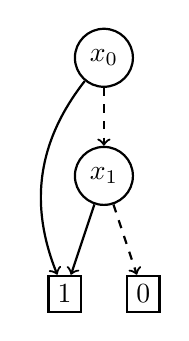
\begin{tikzpicture}
\node[circle, thick, draw] (v4) at (0,3) {$x_0$};
\node[circle, thick, draw] (v1) at (0,1.5) {$x_1$};
\node[rectangle, thick, draw] (v2) at (-0.5,0) {$1$};
\node[rectangle, thick, draw] (v3) at (0.5,0) {$0$};

\draw[->, thick]  (v1) edge (v2);
\draw[->, thick, dashed]  (v1) edge (v3);

\draw[->, thick]  (v4) edge [bend right=30 ] (v2);
\draw[->, thick, dashed]  (v4) edge (v1);

\end{tikzpicture}